
\Section{Payment channels}
One of the biggest problems facing Bitcoin is scalability. At the time of writing
onchain\footnote{See glossary} transactions is capped at about $\approx 7$ T/s (transactions per second).\cite{scaling}
The throughput is limited by network propagation and a hard cap on block sizes, a block
can only contain so many transactions before it is full. There are a couple of
proposed solutions to this however, and one of them is connected payment channels

First off, a payment channel in Bitcoin is a type off trick using programmable transactions, 
were two users can open a bidirectional payment channel where an infinite number of transactions 
could be trustlessly exchanged without using the blockchain. 

A channel can be opend by one or both participants by using a funding transaction. The funding 
transaction requires the signature of both participants to spend and is transmitted to the blockchain. 
After that the participants in the channel exchange commitment transactions that represent exchange in money.
Any of the commitment transactions could be broadcast to the blockchain whenever a participant 
want to close the channel. Once a channel has been closed it cannot be used for further transactions.
Mechanisms exists in the construction of these channels that makes it so one participant 
can't cheat the system and spend money that does not belong to them.

Payment channels alone were not enough to fix the scaling problem however, as a payment channel 
only allows two parties to exchange unlimited transactions. A proposed extension to the 
payment channels is the lightning network.

\Subsection{Lightning network}
Lightning network is a relatively recent development in the Bitcoin community.
How to construct payment channels has been known about for a while. But in
January of 2016 a white paper was released detailing a promising new extension.\cite{lightningnetwork_2019}
It showed that with a few changes to the Bitcoin protocol a new type of
payment channel could be opened that allows transactions to propagate through multiple channels.\cite{lightningnetwork_2019}

\begin{figure}[H]
	\centering
	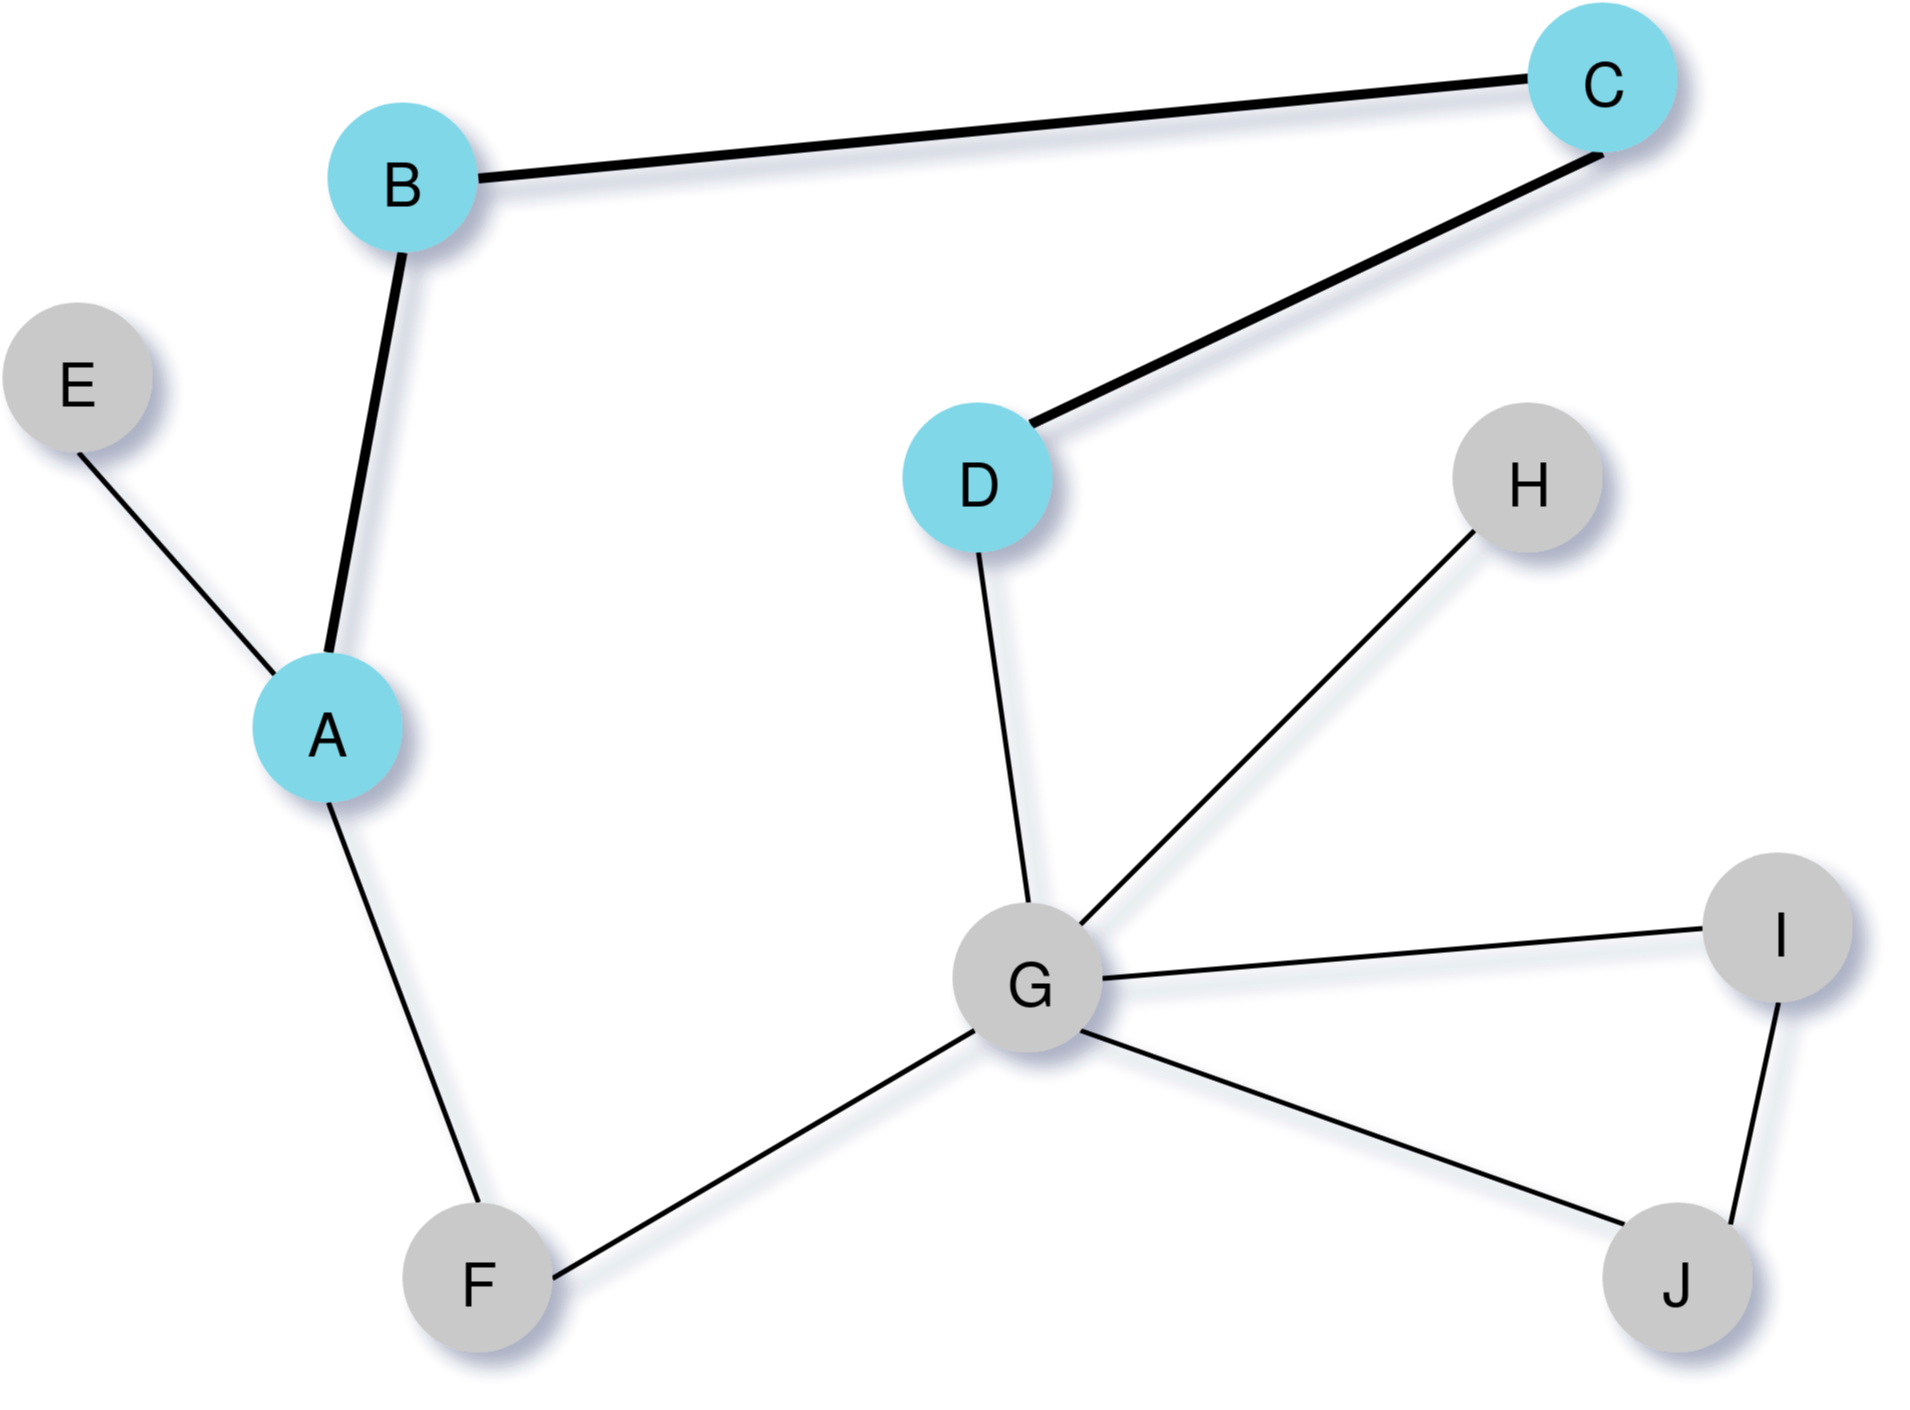
\includegraphics[width=0.70\textwidth]{introduction/images/mesh_network.png}
	\caption{A basic overview of a Lightning network, each node represent someone
	and each edge represents a channel between two people.}
	\label{fig:mesh}
\end{figure}

Lightning network is really just a network of peers connected via payment channels. In figure \ref{fig:mesh} is an example. Let's say that Alice (node A) want to send a transaction to David (node D) but they have no direct payment channel between them. With lightning network they can send the transaction via the peers that are between them, given that there is a path between the nodes, and that there is enough funds in all the channels between. 